\documentclass[11pt]{standalone}
\usepackage{fontspec}
\usepackage{tikz}
\usetikzlibrary{calc,positioning}
\usepackage{xcolor}
\definecolor{bpsnavy}{HTML}{123A6B}
\definecolor{bpsbiru}{HTML}{0B6FB4}
\definecolor{bpsbirumuda}{HTML}{6FB3E0}
\definecolor{bpsoranye}{HTML}{F58220}
\definecolor{bpshijau}{HTML}{00A651}
\definecolor{abuteks}{HTML}{45505C}
\definecolor{abupanel}{HTML}{F1F3F5}
\definecolor{abugaris}{HTML}{C9D1D9}
\definecolor{abujudul}{HTML}{E4E8EC}
\setmainfont{Carlito}
\begin{document}
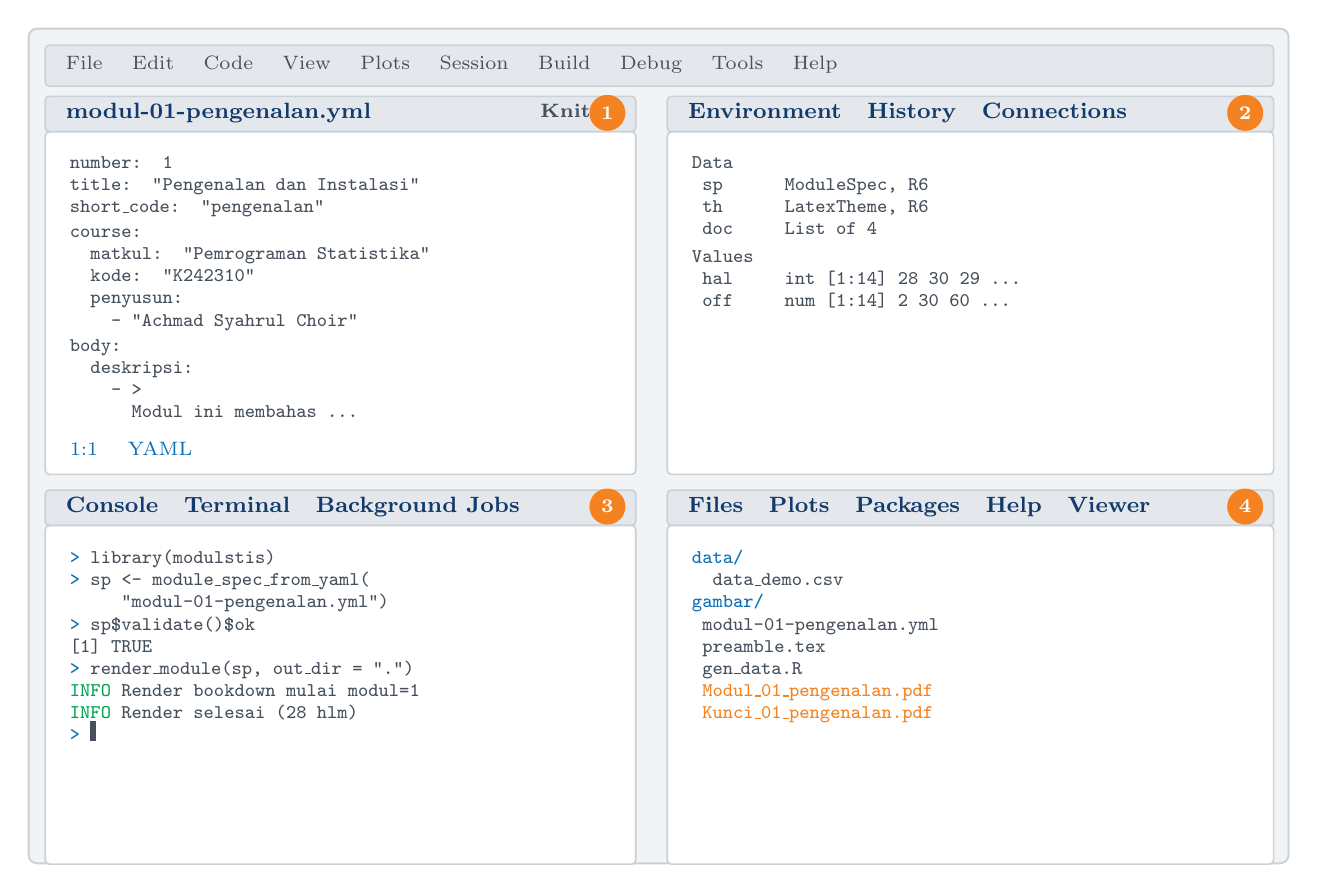
\begin{tikzpicture}[
  panel/.style={draw=abugaris, fill=white, rounded corners=1.5pt, line width=0.6pt},
  judul/.style={draw=abugaris, fill=abujudul, rounded corners=1.5pt, line width=0.6pt},
  tl/.style={font=\footnotesize\bfseries, text=bpsnavy},
  ket/.style={font=\scriptsize, text=abuteks},
  kode/.style={font=\ttfamily\scriptsize, text=abuteks},
  nomor/.style={circle, fill=bpsoranye, text=white, font=\bfseries\scriptsize,
                inner sep=1.6pt, minimum size=13pt}
]
% ---------- bingkai jendela ----------
\fill[abupanel, rounded corners=3pt] (0,0) rectangle (16,10.6);
\draw[abugaris, rounded corners=3pt, line width=0.7pt] (0,0) rectangle (16,10.6);

% bilah menu
\node[judul, minimum width=15.6cm, minimum height=0.52cm, anchor=north west] at (0.2,10.4) {};
\node[ket, anchor=west] at (0.35,10.14)
  {File \quad Edit \quad Code \quad View \quad Plots \quad Session \quad Build \quad Debug \quad Tools \quad Help};

% ---------- kiri atas: Source ----------
\node[judul, minimum width=7.5cm, minimum height=0.45cm, anchor=north west] at (0.2,9.75) {};
\node[tl, anchor=west] at (0.35,9.53) {modul-01-pengenalan.yml};
\node[ket, anchor=east] at (7.6,9.53) {\textbf{Knit} $\;\vert\;$ };
\node[panel, minimum width=7.5cm, minimum height=4.35cm, anchor=north west] at (0.2,9.3) {};
% isi editor: cuplikan YAML
\node[kode, anchor=north west, align=left] at (0.4,9.1)
  {number: 1\\
   title: "Pengenalan dan Instalasi"\\
   short\_code: "pengenalan"\\[1pt]
   course:\\
   \ \ matkul: "Pemrograman Statistika"\\
   \ \ kode: "K242310"\\
   \ \ penyusun:\\
   \ \ \ \ - "Achmad Syahrul Choir"\\[1pt]
   body:\\
   \ \ deskripsi:\\
   \ \ \ \ - >\\
   \ \ \ \ \ \ Modul ini membahas ...};
\node[ket, anchor=south west, text=bpsbiru] at (0.4,5.05) {1:1 \quad YAML};

% ---------- kanan atas: Environment ----------
\node[judul, minimum width=7.7cm, minimum height=0.45cm, anchor=north west] at (8.1,9.75) {};
\node[tl, anchor=west] at (8.25,9.53) {Environment \; History \; Connections};
\node[panel, minimum width=7.7cm, minimum height=4.35cm, anchor=north west] at (8.1,9.3) {};
\node[kode, anchor=north west, align=left] at (8.3,9.1)
  {\textbf{Data}\\
   \ sp \ \ \ \ \ ModuleSpec, R6\\
   \ th \ \ \ \ \ LatexTheme, R6\\
   \ doc \ \ \ \ List of 4\\[2pt]
   \textbf{Values}\\
   \ hal \ \ \ \ int [1:14] 28 30 29 ...\\
   \ off \ \ \ \ num [1:14] 2 30 60 ...};

% ---------- kiri bawah: Console ----------
\node[judul, minimum width=7.5cm, minimum height=0.45cm, anchor=north west] at (0.2,4.75) {};
\node[tl, anchor=west] at (0.35,4.53) {Console \; Terminal \; Background Jobs};
\node[panel, minimum width=7.5cm, minimum height=4.3cm, anchor=north west] at (0.2,4.3) {};
\node[kode, anchor=north west, align=left] at (0.4,4.1)
  {\textcolor{bpsbiru}{>} library(modulstis)\\
   \textcolor{bpsbiru}{>} sp <- module\_spec\_from\_yaml(\\
   \ \ \ \ \ "modul-01-pengenalan.yml")\\
   \textcolor{bpsbiru}{>} sp\$validate()\$ok\\
   {[}1{]} TRUE\\
   \textcolor{bpsbiru}{>} render\_module(sp, out\_dir = ".")\\
   \textcolor{bpshijau}{INFO} Render bookdown mulai modul=1\\
   \textcolor{bpshijau}{INFO} Render selesai (28 hlm)\\
   \textcolor{bpsbiru}{>} \rule{2pt}{7pt}};

% ---------- kanan bawah: Files/Plots/Viewer ----------
\node[judul, minimum width=7.7cm, minimum height=0.45cm, anchor=north west] at (8.1,4.75) {};
\node[tl, anchor=west] at (8.25,4.53) {Files \; Plots \; Packages \; Help \; Viewer};
\node[panel, minimum width=7.7cm, minimum height=4.3cm, anchor=north west] at (8.1,4.3) {};
\node[kode, anchor=north west, align=left] at (8.3,4.1)
  {\textcolor{bpsbiru}{\textbf{data/}}\\
   \ \ data\_demo.csv\\
   \textcolor{bpsbiru}{\textbf{gambar/}}\\
   \ modul-01-pengenalan.yml\\
   \ preamble.tex\\
   \ gen\_data.R\\
   \ \textcolor{bpsoranye}{Modul\_01\_pengenalan.pdf}\\
   \ \textcolor{bpsoranye}{Kunci\_01\_pengenalan.pdf}};

% ---------- penanda bernomor ----------
\node[nomor] at (7.35,9.53) {1};
\node[nomor] at (15.45,9.53) {2};
\node[nomor] at (7.35,4.53) {3};
\node[nomor] at (15.45,4.53) {4};
\end{tikzpicture}
\end{document}
